\section{Security Orchestration Automation and Response}

The increasing volume, velocity, and sophistication of cyber threats have made manual incident response insufficient in modern Security Operations Centers (SOCs). As organizations face growing pressure to detect and mitigate attacks in real time, Security Orchestration, Automation, and Response (SOAR) platforms have emerged as a critical solution for scaling security operations and reducing response times. SOAR systems integrate threat intelligence, automate repetitive tasks, and orchestrate incident handling workflows across various tools and teams~\cite{paloalto_soar, ibm_soc}.

This internship project, conducted at Bharat Electronics Limited (BEL), focuses on the design and implementation of a custom SOAR platform tailored for real-time cyber incident management. The platform includes core modules such as user authentication, an interactive dashboard, incident analytics, workflow automation, playbook execution, and integration with the MITRE ATT\&CK framework~\cite{mitre_attack}. The goal is to reduce Mean Time to Detect (MTTD) and Mean Time to Respond (MTTR) by enabling rapid triage and automated mitigation.

By integrating automation driven decision support with customizable workflows, this SOAR platform empowers security analysts to respond proactively to threats while minimizing fatigue and human error. The project aligns with industry best practices and addresses real-world challenges in enterprise-grade SOC environments.

\section*{Security Operations Center (SOC) and the Role of SOAR}

A Security Operations Center (SOC) is a centralized facility responsible for continuously monitoring, detecting, analyzing, and responding to cybersecurity incidents within an organization. SOC teams play a critical role in safeguarding information systems by managing security alerts, coordinating incident responses, and maintaining compliance with organizational and regulatory policies~\cite{ibm_soc}.

Typically, a SOC is staffed with multiple tiers of security analysts:
\begin{itemize}[noitemsep, topsep=0pt]
    \item \textbf{Tier 1 (Alert Analysts):} Responsible for monitoring alerts, triaging incidents, and escalating suspicious activities.
    \item \textbf{Tier 2 (Incident Responders):} Perform deeper investigations, validate threats, and initiate containment actions.
    \item \textbf{Tier 3 (Threat Hunters):} Conduct proactive threat hunting and in-depth forensic analysis.
\end{itemize}

\begin{figure}[htbp]
    \centering
    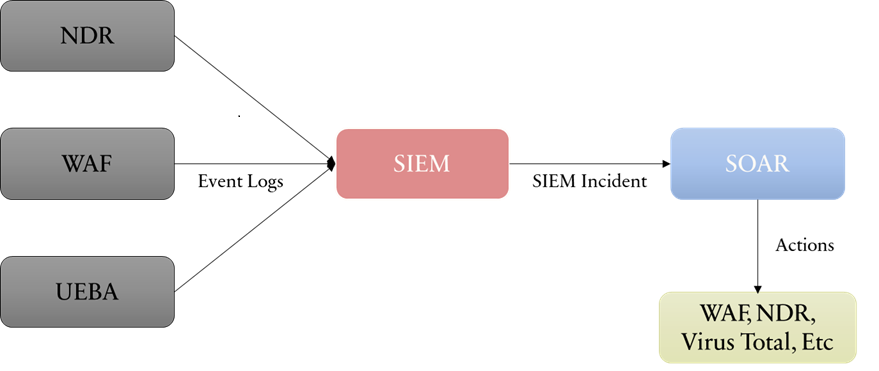
\includegraphics[width=0.85\textwidth]{images/data_flow_soc.png}
    \caption{Data flow in a typical Security Operations Center (SOC) environment.}
    \label{fig:data_flow_soc}
\end{figure}

However, as cyberattacks grow more sophisticated and the volume of alerts increases, traditional SOCs face challenges related to analyst fatigue, delayed response times, and inconsistent incident handling. This is where SOAR (Security Orchestration, Automation, and Response) platforms play a transformative role.

SOAR systems integrate with SIEM (Security Information and Event Management) tools, threat intelligence platforms, and endpoint security solutions to automate repetitive tasks, correlate events across systems, and trigger predefined playbooks. This reduces Mean Time to Detect (MTTD) and Mean Time to Respond (MTTR), while also ensuring standardization and auditability of incident response actions~\cite{paloalto_soar}.

In this project, the SOAR platform was designed to emulate real SOC workflows, enabling seamless analyst interaction, intelligent response orchestration, and alignment with the MITRE ATT\&CK framework~\cite{mitre_attack}, thereby enhancing the operational efficiency of the SOC environment.

\section*{SOAR Platform Components}
\addcontentsline{toc}{section}{SOAR Platform Components}

The custom SOAR platform developed during this internship consists of multiple integrated components designed to streamline and automate cybersecurity operations. Each module is built with a focus on usability, scalability, and alignment with real-world SOC workflows. The primary components are as follows:

\begin{enumerate}
    \item \textbf{User Authentication and Access Control:} 
    Implements secure login and registration with role-based access to differentiate between analysts, administrators, and managers.

    \item \textbf{Dashboard and Incident Analytics:} 
    Provides real-time visualizations including pie charts (severity, status), bar graphs (top events), and time-series graphs to track incident trends and mitigation rates.

    \item \textbf{Incident Management Module:} 
    Displays a dynamic table of security incidents enriched with deatils about the incident. Analysts can manually review, assign, and change incident statuses or let the system apply automated mitigation using machine learning.

    \item \textbf{Integrations Module:} 
    Enables external application integration via RESTful APIs. Users can configure apps (name, token, description) and their corresponding actions (endpoint, method, parameters).

    \item \textbf{Playbook Management:} 
    Supports creation and editing of automated response playbooks triggered by MITRE ATT\&CK technique IDs. Each playbook is mapped to workflows for seamless execution.

    \item \textbf{Workflow Builder:} 
    Offers a drag-and-drop interface to define logical sequences of actions using app nodes and edges. Analysts can design, execute, and track workflows in real time.

    \item \textbf{MITRE ATT\&CK Matrix Integration:} 
    Visualizes ATT\&CK techniques, allowing analysts to explore incident frequency and identify attack vectors. Techniques are color-coded based on activity density.

\end{enumerate}

These components collectively enable end-to-end incident response orchestration, minimize analyst fatigue, and improve SOC efficiency through intelligent automation.
